\documentclass{article}


% if you need to pass options to natbib, use, e.g.:
%     \PassOptionsToPackage{numbers, compress}{natbib}
% before loading neurips_2022


% ready for submission
%\usepackage{neurips_2022}


% to compile a preprint version, e.g., for submission to arXiv, add add the
% [preprint] option:
\usepackage[preprint, nonatbib]{neurips_2022}


% to compile a camera-ready version, add the [final] option, e.g.:
%     \usepackage[final]{neurips_2022}


% to avoid loading the natbib package, add option nonatbib:
%    \usepackage[nonatbib]{neurips_2022}


\usepackage[utf8]{inputenc} % allow utf-8 input
\usepackage[T1]{fontenc}    % use 8-bit T1 fonts
\usepackage{hyperref}       % hyperlinks
\usepackage{url}            % simple URL typesetting
\usepackage{booktabs}       % professional-quality tables
\usepackage{amsfonts}       % blackboard math symbols
\usepackage{nicefrac}       % compact symbols for 1/2, etc.
\usepackage{microtype}      % microtypography
\usepackage{xcolor}         % colors

\usepackage{biblatex}
\addbibresource{neurips_2022.bib}
\usepackage{pythonhighlight}
\usepackage{graphicx}

\title{Computer Vision Proseminar Report WS2023}


% The \author macro works with any number of authors. There are two commands
% used to separate the names and addresses of multiple authors: \And and \AND.
%
% Using \And between authors leaves it to LaTeX to determine where to break the
% lines. Using \AND forces a line break at that point. So, if LaTeX puts 3 of 4
% authors names on the first line, and the last on the second line, try using
% \AND instead of \And before the third author name.


\author{%
    Markus Diller\\
    University of Salzburg\\
    Salzburg, 5020 \\
    \texttt{markus.diller@stud.plus.ac.at} \\
    \And
    Marcel Sargant \\
    University of Salzburg \\
    Salzburg, 5020 \\
    \texttt{marcel.sargant@stud.plus.ac.at} \\
}


\begin{document}


\maketitle


\begin{abstract}
    The aim of this report is to investigate the ConvNeXt network architecture and its components and try it with the CIFAR10 dataset.
    For that we used an already existing implementation that was built around and evaluated on the ImageNet1k dataset.
    Therefore, we played around with the mechanisms used in the implementation such as data augmentation, finetuning and the network architecture itself.
    What we concluded in our findings is that it works very well when using a pretrained model but only moderately well when training from scratch.
\end{abstract}


\section{Introduction}\label{sec:introduction}
In this proseminar we have been tasked with familiarizing ourselves with an existing implementation of a neural network architecture.
The network in question is the ConvNeXt architecture developed by \textit{facebookresearch} and published in 2022.
In the associated paper the authors present their methodology and design decisions.
While the authors get interesting results, they only apply to the ImageNet1k dataset.
Therefore, to truly understand the architecture and see how well it works with another dataset we experimented with using the CIFAR10 dataset.

This report first summarizes the key aspects presented in the ConvNeXt paper as well as presents the experiments we did using the implementation.
These experiments can be grouped into three categories that are data augmentation, finetuning and reverting network structures.
Finally, in the end we will draw conclusions about our findings.

\section{ConvNeXt}\label{sec:convnext}
% summarize the key aspects of the paper, 1 - 1.5p
ConvNeXt\cite{liu2022convnet} is the label for a machine learning project of Liu, Mao et al., regarding image classification.
It is supposed to show an alternative to the in machine learning science currently mainly focussed vision transformers.
To achieve this, they start with a standard ResNet and modify it with techniques used or developed in vision transformers and optimize training and model parameters in respect to maximum accuracy.

One of the most famous image classification models is the ResNet, using conventional convolution layers, reaching high scores in terms of accuracy and being base model for multiple other ConvNets.
It is available in different variants, defined by the structural depth.
For ConvNeXt both, the ResNet-50 with around 4.5e9 FLOPs and ResNet-200 having around 15e9 FLOPs are used and compared with different parameters.
On the counterpart, looking at transformers, they originally abandon any convolutions, ConvNext implements design principles of the Swin Transformer that combines the transformers technology and convolutions, to achieve higher accuracy and comparing it to the accuracy of the standard Swin Transformer.
The derivatives used are Swin-T and Swin-B for ResNet-50 and ResNet-200 respectively.
Besides that, ConvNeXt uses an adapted set of training parameters like an increased number of epochs, a special set of data augmentation and the AdamW optimizer.

As we will discuss each of the reversions done for ConvNeXt later, we will now briefly go through the most important adaptions made in comparison to a standard ResNet.

\textbf{Shape.}
While ResNet-50 uses a stage compute ratio of (3,4,6,3), Swin Transformers have a ratio of 1:1:9:1.
In ConvNeXt, the shape is set to (3,3,9,3)

\textbf{Patchify.}
Opposing traditional ConvNet designs, vision transformers do not use overlapping kernels in the convolution input layers, but instead non overlapping, usually larger kernels.
ConvNeXt keeps small kernels but does not let them overlap, reaching even slightly better results with this simplification.

\textbf{ResNeXt-ify.}
The Network ResNeXt works with grouped convolution, i.e.\ grouping convolutional filters.
ConvNeXt uses similar depth wise convolution which is a special case of grouped convolution.

\textbf{Inverted Bottleneck.}
As used in Transformers, ConvNeXt uses an inverted bottleneck, i.e.\ the dimension of the hidden convolution layer is increased by a ratio of 4.
Although this inverted bottleneck has more FLOPs because of the used depth wise convolution layer, overall FLOPs drop, as the used 1x1 convolution Layers reduce the FLOPs drastically (for layer structure see \autoref{fig:bottleneck})
\begin{figure}[h]
    \centering
    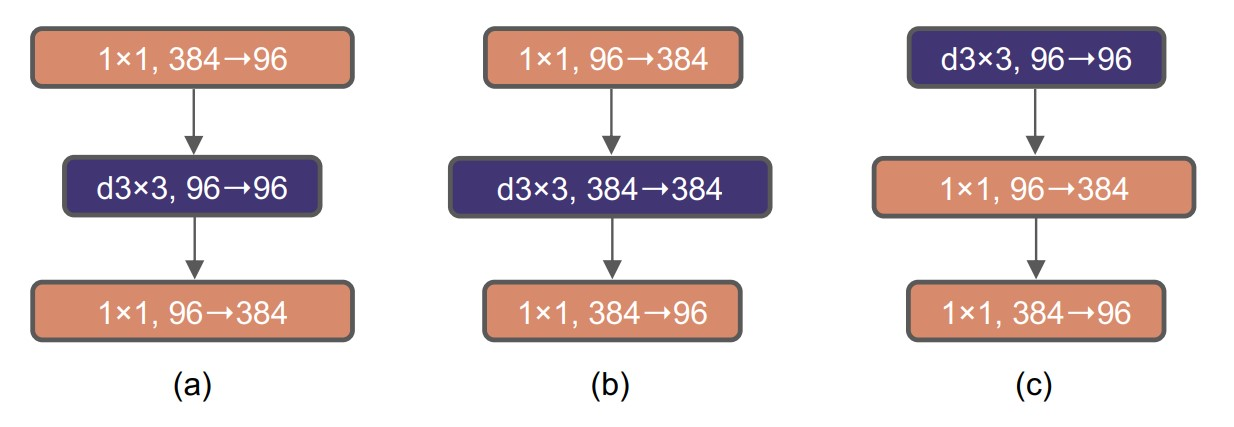
\includegraphics[width=0.7\textwidth]{images/bottleneck}
    \caption{Evolution of the Bottleneck\cite{liu2022convnet}}
    \label{fig:bottleneck}
\end{figure}

\textbf{Large Kernel sizes.}
Another key feature of transformers is that its layers have global reception.
In order to approximate this approach, ConvNeXt runs with increased sized kernels, going up to 7x7 which is also the minimum size in Swin Transformers.

\textbf{Other Minor changes.}
\begin{itemize}
    \item Using the GELU activation function which operates slightly smoother then ReLU and is used in multiple famous transformers.
    \item Reduced number of activation functions.
    \item Reduced number of normalization layers.
    \item Using the simpler Layer Normalization instead of BatchNorm.
    \item Using separate down-sampling layers with stabilizing LNs respectively.
\end{itemize}


\section{Documentation}\label{sec:documentation}
For our work with the ConvNeXt architecture we investigated three main ideas.
The first and most thorough was the effect of data augmentation on the network performance.
The second was to experiment with the finetuning provided by the given implementation.
Finally, the third focus was to revert some of the changes~\Citeauthor{liu2022convnet} made to the ResNet they built upon.

As it is always a difficult choice to pick the hyperparameters, in our experiments we just used two different configurations that henceforth will be called \texttt{paper} and \texttt{example}, respectively.
The first set was taken from the second column in Table 5 of the ConvNeXt\cite{liu2022convnet} paper and the second were taken from the example Colab project presented on the networks GitHub page\cite{ayush0finetune}.
\autoref{tab:hyperparameters} shows all hyperparameters that are not set to the default values.
We also always chose the tiny ConvNeXt model.
What additionally differs from the setup in the paper is the dataset used.
Instead of ImageNet1k all our training runs are based on the CIFAR10\cite{krizhevsky2009learning} dataset reduced to 10\% of its original size.
Also, the implementation uses a fixed seed, therefore the results should be deterministic and reproducible.
The networks were trained on three different machines, which roughly took the same magnitudes for training.
These are an Nvidia RTX 3070, an Nvidia RTX 3060 mobile, and the opaque Google Colab T4 GPU\@.
Both the ConvNeXt implementation and CIFAR10 use the MIT license.
\begin{table}[h]
    \caption{Choice of hyperparameters.}
    \begin{center}
        \begin{tabular}{lll}
            \hline
            Parameter     & \texttt{paper} & \texttt{example} \\ \hline
            learning rate & 4e-3           & 4e-4             \\
            warmup epochs & 5              & 0                \\
            cutmix        & 1              & 0                \\
            mixup         & 0.8            & 0                \\
            EMA decay     & 1              & 0.9999
        \end{tabular}
    \end{center}
    \label{tab:hyperparameters}
\end{table}

\subsection{Code Modification and Quality of Life}\label{subsec:code-modification}
To allow for an improved workflow for testing we chose to make some minor changes to the given codebase.
This was done to not only ensure faster training times, but also for a more lenient experience when having to set up the environment.

The first and only change that meddles with the actual implementation was to add another command line argument to allow for down-sampling CIFAR10.
For this we registered a \texttt{--downsample} argument to the used argparser that is then used in the \verb|build_dataset| function in the \texttt{dataset.py} file.
The implementation for the usage can be seen in~\ref{fig:downsampling}.
Instead of choosing a random subset we choose every $n$th element, where $n$ is the down-sampling factor.
Additionally, for transparency, the original codebase used CIFAR100, but we chose to change it to CIFAR10.
\begin{figure}[h]
    \begin{python}
        dataset = datasets.CIFAR10(args.data_path, train=is_train,
        transform=transform, download=True)
        sample = list(range(0, len(dataset), args.downsample))
        dataset = torch.utils.data.Subset(dataset, sample)
        nb_classes = 10
    \end{python}
    \caption{Downsampling the dataset.}
    \label{fig:downsampling}
\end{figure}

The second and final change was to create a \texttt{requirements.txt} file for easy installation of the necessary packages.
Due to the codebase being incompatible with versions of pytorch larger than 2.0 and Google Colab defaulting to such a version we created this file to easily install all necessary dependencies with a single command.
This comes especially in handy because Colab resets the runtime after just a few hours of inactivity, in turn also resetting the changes in installed packages.
It eludes us as to why there was no such file already included in the codebase, just a very bare-bones markdown file with requirements.

\subsection{Data Augmentation}\label{subsec:data-augmentation}
The subsampling helped massively in decreasing the training time, but still just taking 10\% of the dataset for training took three hours to train for 100 epochs on our machines and in Google Colab.
We identified that the largest time during training was spent applying transforms to the images.
Therefore, a large focus working with this network architecture was on trying to find a sweet spot between transforms and model accuracy.

Before being able to evaluate the performance of different configurations of image transforms, we need some kind of baseline.
Hence, we first trained the ConvNeXt network as is first with the paper parameters (\texttt{example\_imagenet}) and example parameters (\texttt{example\_imagenet}).
As the example parameters give significantly better results, all future tests will use their hyperparameter configuration.
Additionally, we chose to change the mean and standard deviation used for the normalization transform to the ones from CIFAR10 instead of Imagenet1k (\texttt{from-scratch}).
The values were not calculated by us, but taken from a StackOverflow\cite{stackoverflow} comment.
The resulting accuracy is lower than that when using the initial values, but we prefer proper values over a few more percent accuracy.
The testing accuracy curves of the different configurations can be seen in \autoref{fig:data-augmentation}.

With a baseline of about 65\% accuracy established we can now start to experiment with the image transforms.
We did this by removing it entirely and reintroducing it in steps with minimal changes in the codebase.
One was always necessary, that being the \texttt{ToTensor()} transform as otherwise the training would not even work.
The result was very fast, taking about only five minutes, but had abysmal performance (\texttt{only-totensor}).
This was very suspicious, and we came to find that the testing procedure used different transforms that include a resize.
Therefore, we trained the network on 32 by 32 images and tested it on 224 by 224 images.
Using the \texttt{input\_size} command line argument we can change this behaviour to also testing on the proper image size.
Still, the accuracy (\texttt{only-totensor\_input-is-32}) is very bad.

Something that rubbed us the wrong way during the tests before resizing was that the network seemed to don't mind whether the images were 32 by 32 or 224 by 224.
The linear layer in the implementation has a fixed value for its input dimensions and the images are indeed their specified size when entering the network.
After a bit of digging we found the reason why it did not matter.
After the convolution layers the shape of the data is still different between different image sizes, however, the number of channels is the same.
In a final step before the classification global average pooling is applied that results in the output shape just being batch size and number of channels.

Next, we introduced normalization which only minimally impacted training time, but increased the performance by another 10\% (\texttt{normalize\_input-is-32}).
This was still too bad for us to consider as a worth tradeoff, hence we introduced the resizing back to 224 by 224 pixel images (\texttt{resize}).
The resizing pushed our training time back into more than one hour but achieved performance comparable to the paper parameters.
However, this was still not satisfactory performance wise, and therefore we moved on to playing with the command line arguments for the transforms, as introducing other transforms would modify the codebase too much.
The relevant options one can disable via passing arguments to the model is color jitter, auto augmentation and random erasure.
Other modifications like horizontal flipping and random cropping cannot be disabled without tampering with the code.
Because the documentation of the arguments was so poor in our next test we only managed to disable color jitter, which we found out is always disabled as long as any auto augmentation was done, and random erasure.
We only managed to change the default Random Augment to Auto Augment using the Auto Augment flag.
To our surprise, this configuration (\texttt{cli-augment-off-but-aa}) gave better results than the example parameters whilst also needing half an hour less to train.
The final configuration we tested was to properly disable the auto augmentation as well (\texttt{cli-augment-off}).
The results were also better than the example parameters, but slightly worse than the prior configuration while having no change in training time.

The conclusion of these experiments was that we can improve the performance of training from scratch by varying the command line arguments but not the training time.
Hence, in the coming chapters we will use it in tandem with the example parameter configuration for testing when wanting to squeeze out a bit more performance.
\begin{figure}[h]
    \centering
    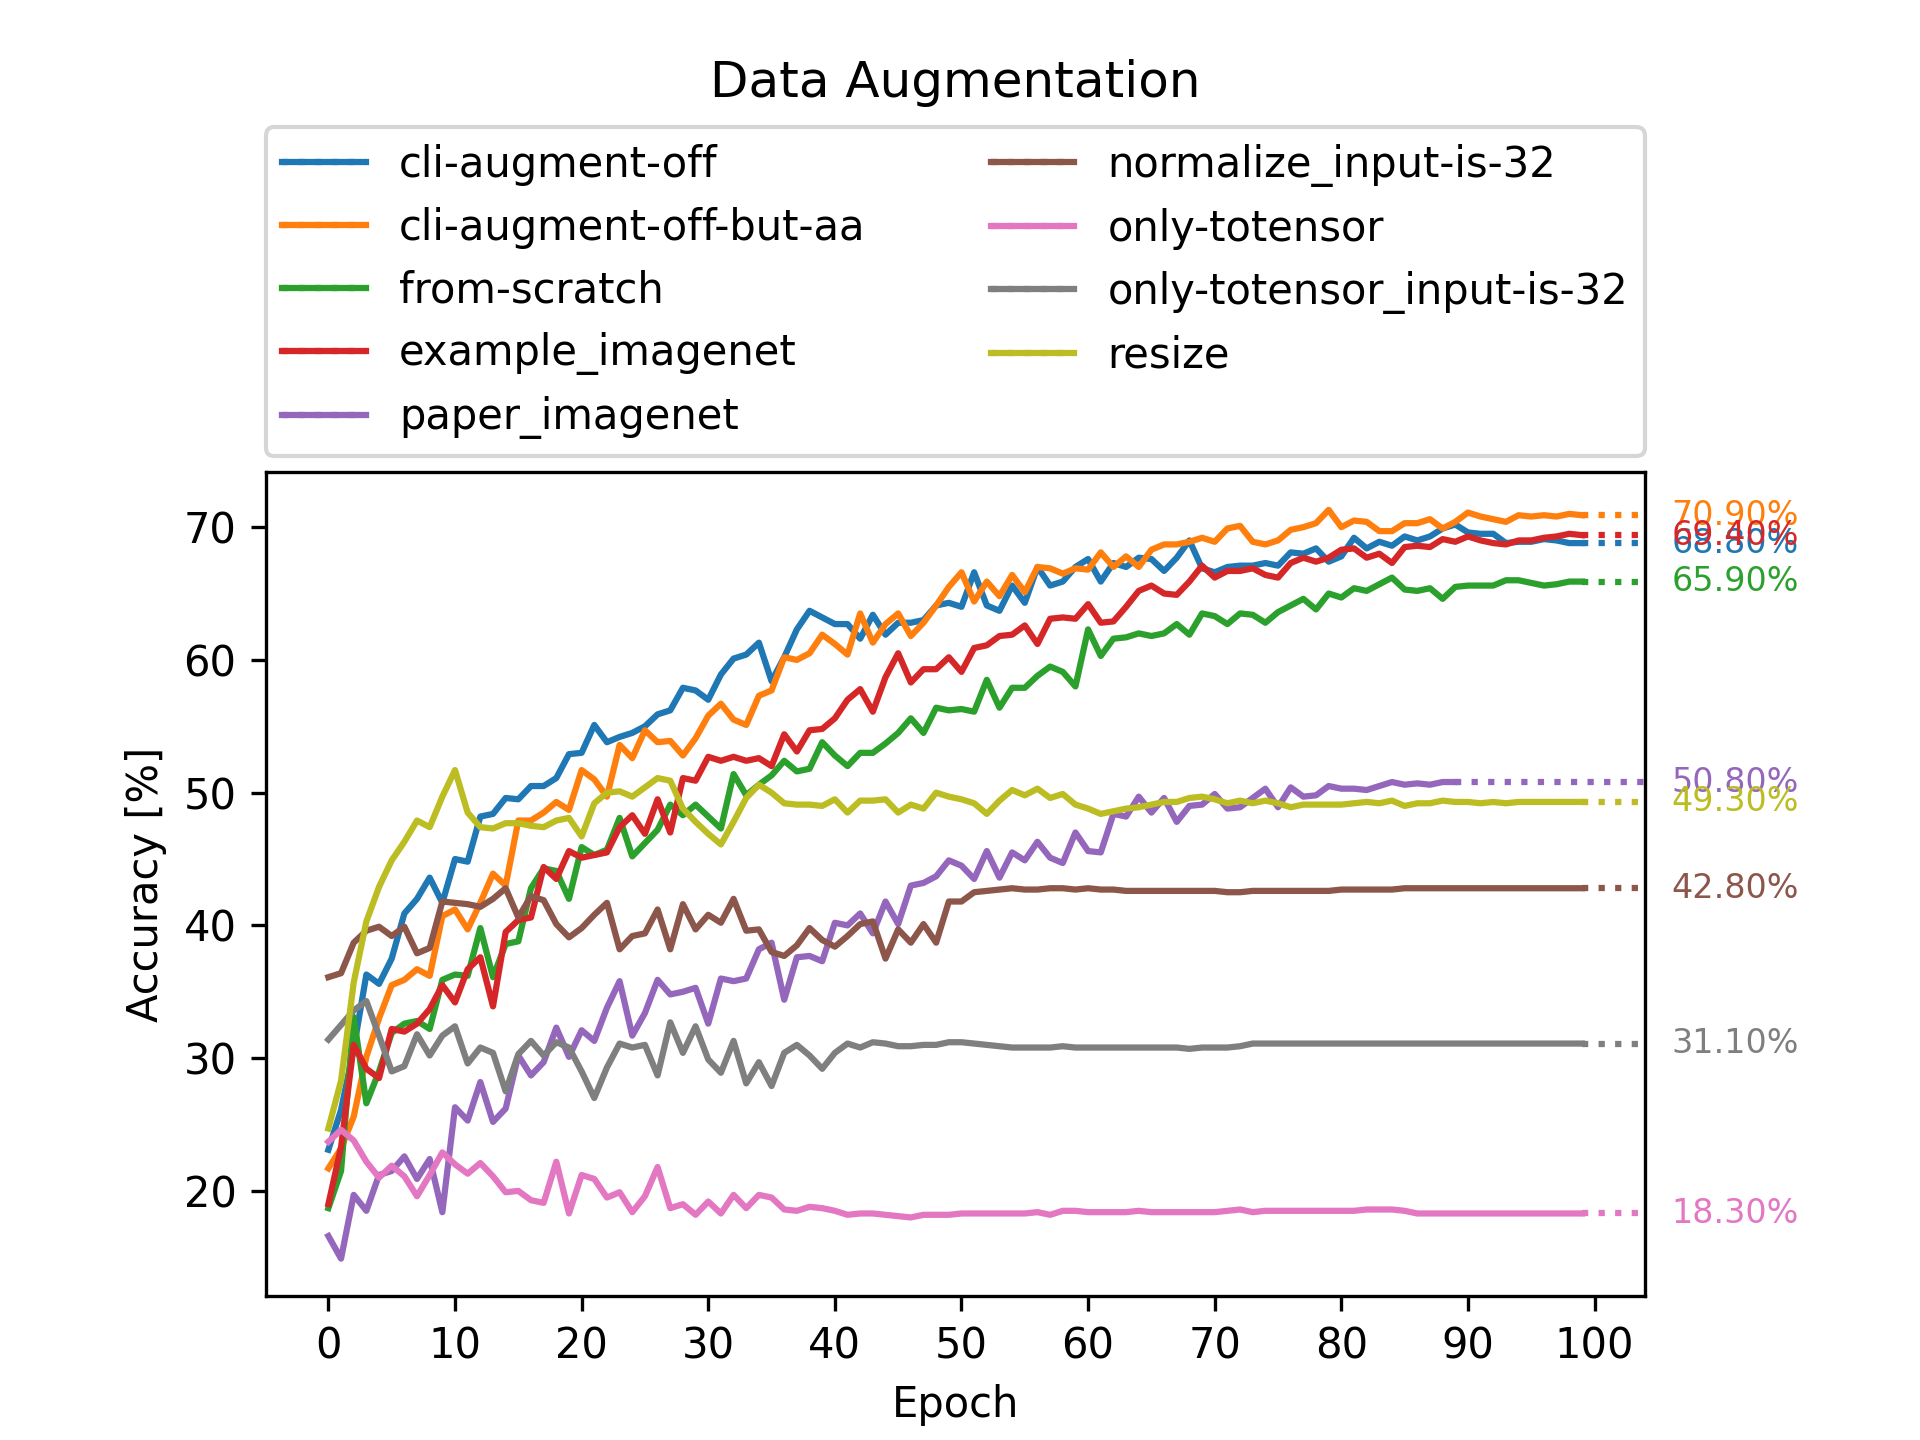
\includegraphics[width=0.8\textwidth]{images/data_augmentation}
    \caption{Comparison of different data augmentation configurations.}
    \label{fig:data-augmentation}
\end{figure}

After experimenting with the augmentation, we wanted to see how the images looked after being transformed.
\autoref{fig:image-transforms} shows the different transform configurations being applied to a selection of images.
The first row are the original images resized to 224 by 224 with bicubic interpolation.
The next row depicts the transforms being applied when not changing anything in the command line parameters.
Thirdly, are the images generated when disabling all command line arguments but the auto augmentation.
In the final row all transforms able to be disabled in the command line are displayed.
\begin{figure}[h]
    \centering
    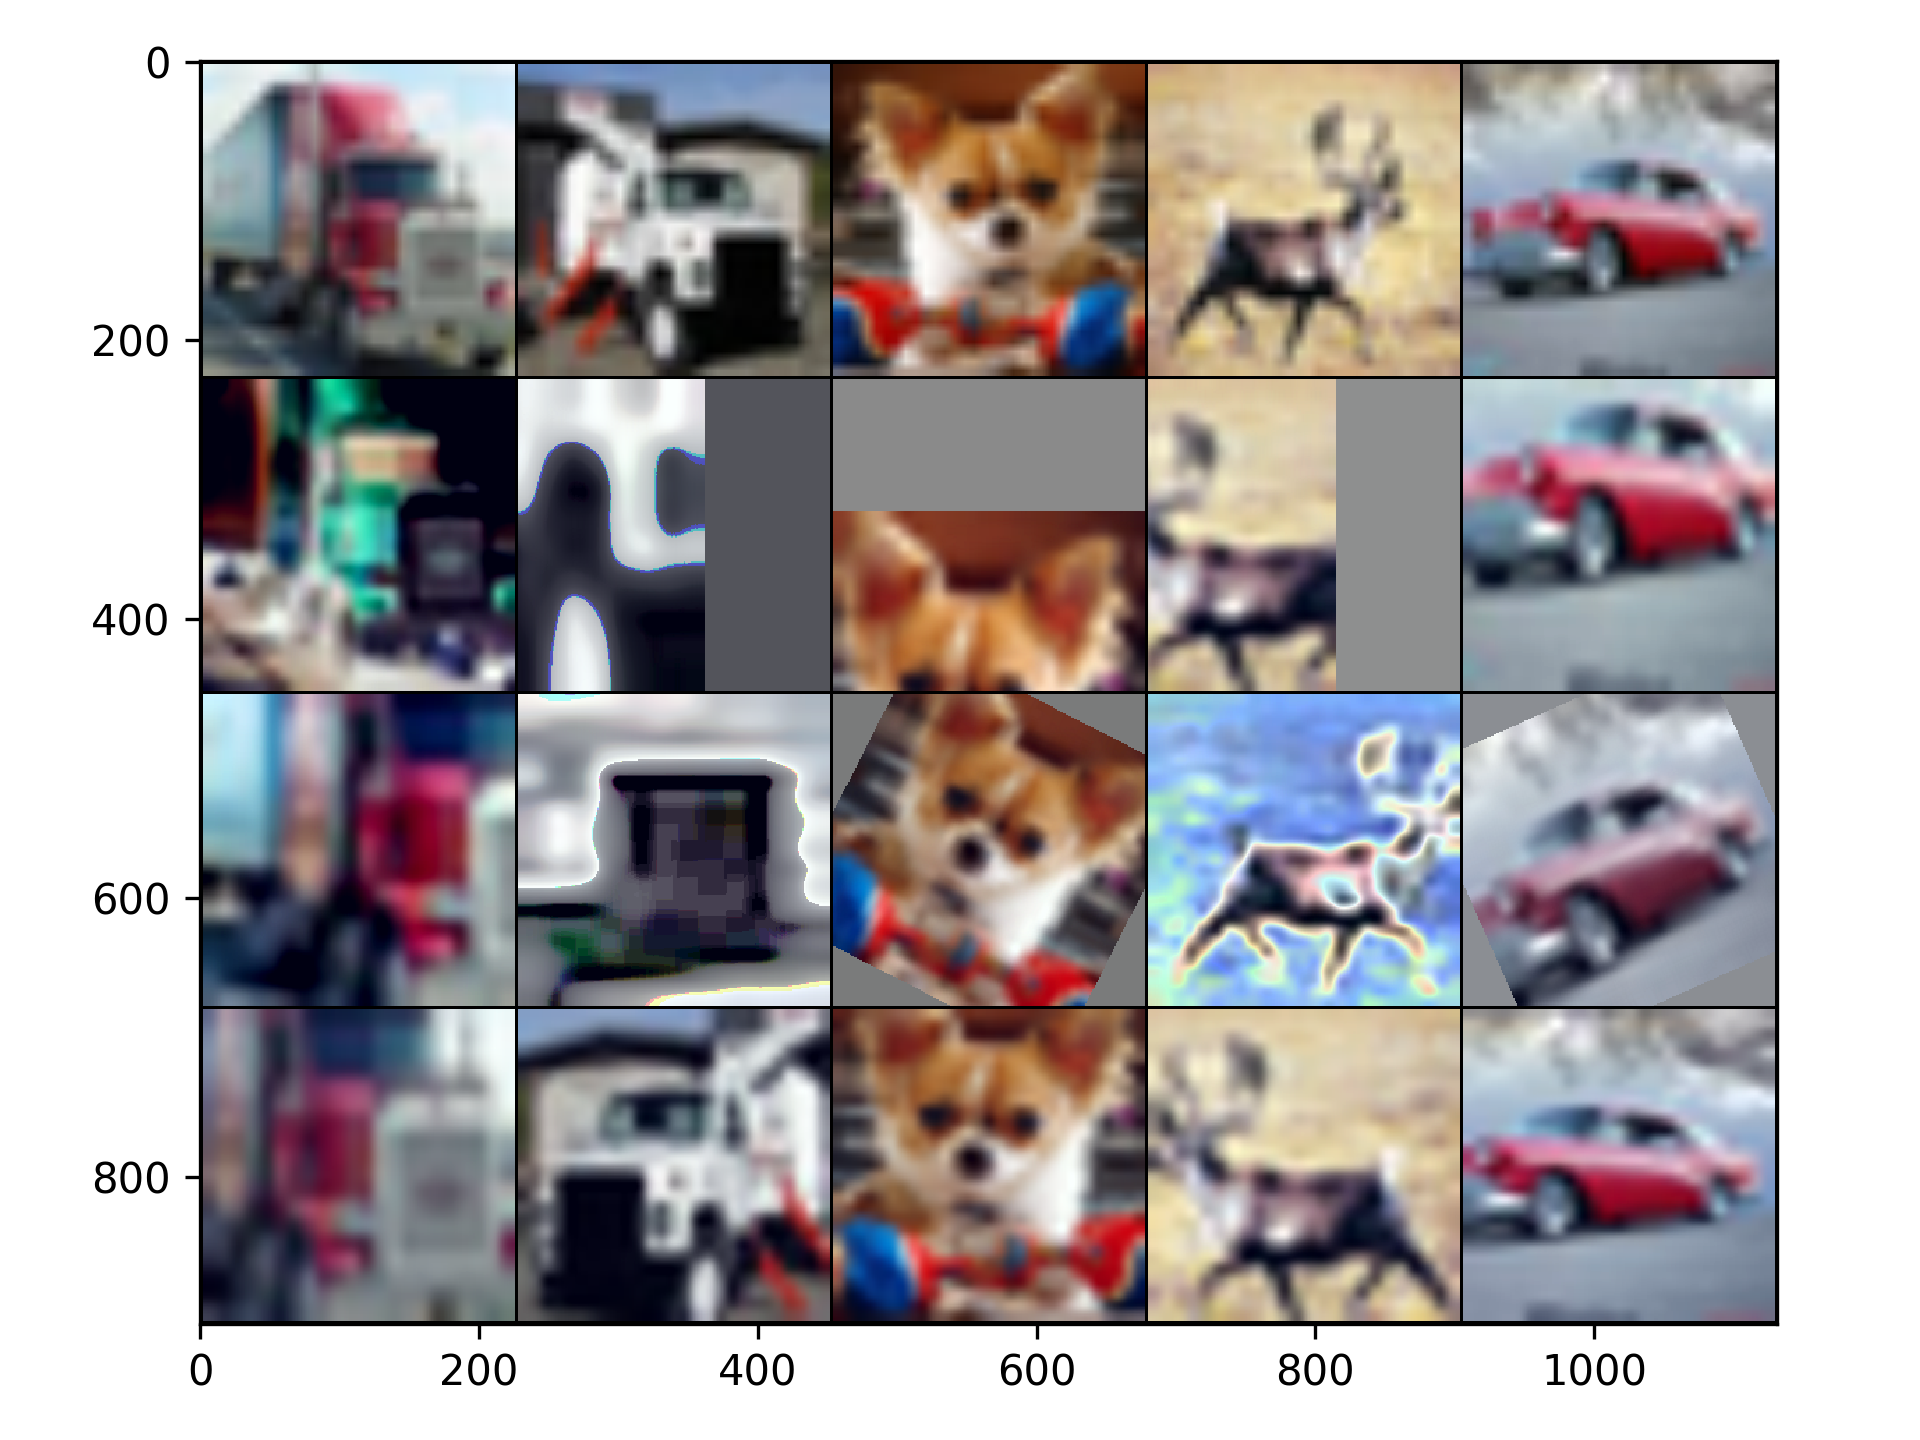
\includegraphics[width=0.7\textwidth]{images/image_transforms}
    \caption{Impact of image transforms on dataset.}
    \label{fig:image-transforms}
\end{figure}

\subsection{Finetuning}\label{subsec:finetuning}
During our trials for improved training time we also experimented with the finetuning in the network.
It was astounding that just using the command in~\cite{ayush0finetune} we managed to achieve an accuracy of 95\% (\texttt{finetune}) even though for training from scratch we capped at 70\%.
Therefore, our goal was to try and squeeze out as much performance as possible.
The results for our finetuning can be seen in \autoref{fig:finetuning} and the configurations will be explained in the next paragraphs.
\begin{figure}[h]
    \centering
    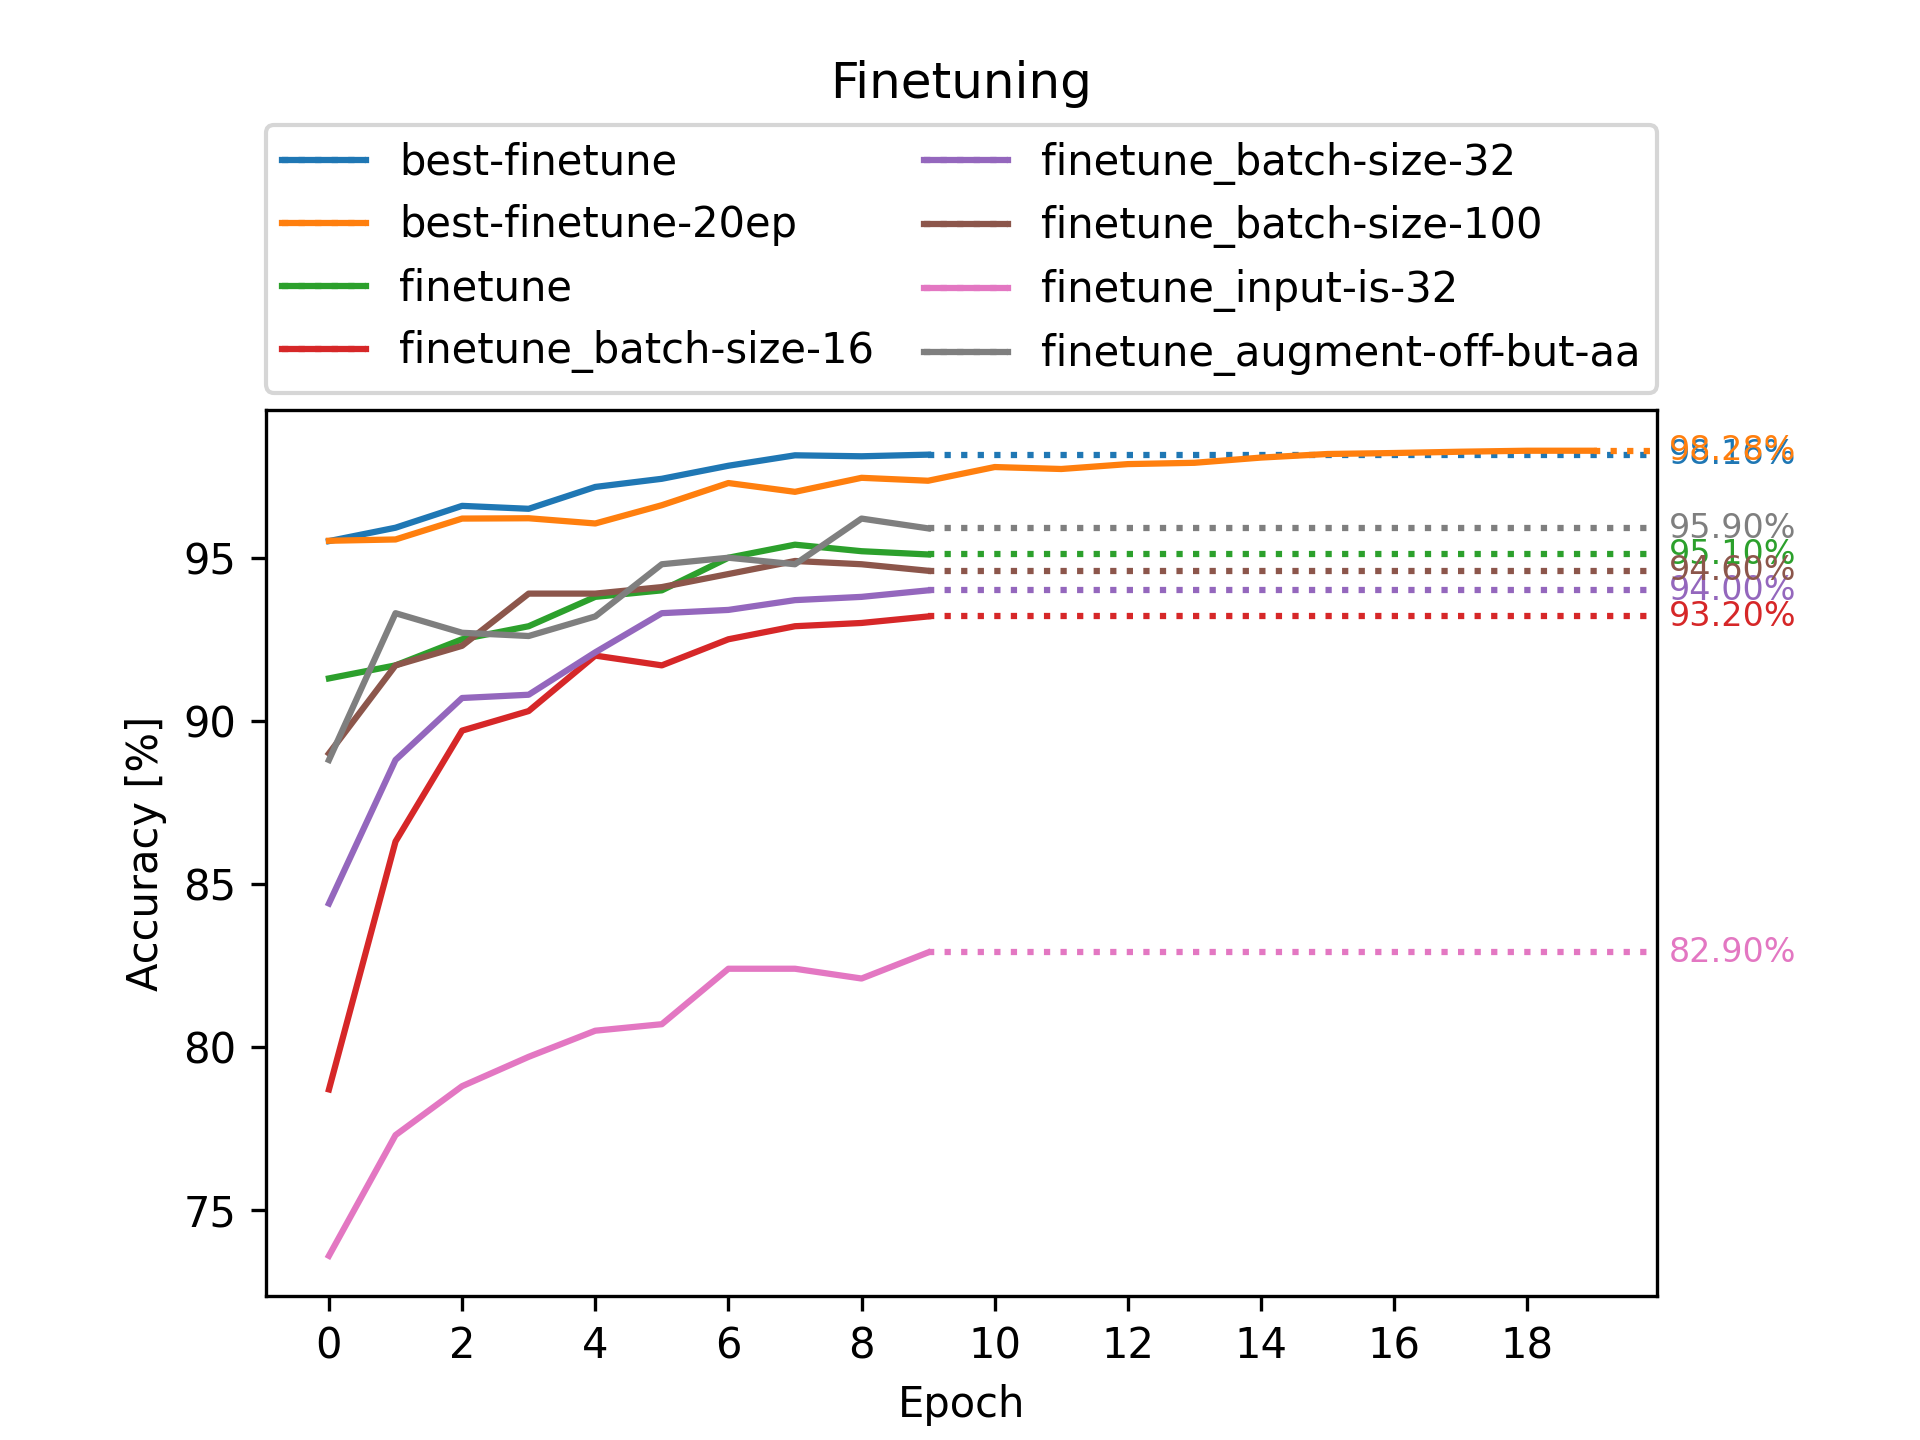
\includegraphics[width=0.8\textwidth]{images/finetuning}
    \caption{Comparison of finetuning configurations.}
    \label{fig:finetuning}
\end{figure}

For our finetuning instead of training for 100 epochs, we only trained for 10, except in one case.
We always chose the example parameters and fine-tuned the pretrained ConvNeXt-T for ImageNet-1K model\cite{repository}.
Finetuning can be initiated by specifying a reference to a pretrained model, in our case a link, as a command line parameter with the \texttt{--finetune} option.

We did three different sets of tests when it came to finetuning in order to squeeze out performance.
None of these included varying any hyperparameter, other than our first test with different batch sizes.
On our local machine, the maximum amount of video memory was eight gigabytes.
As a result, locally, we were limited to a batch size of 64.
We tried out different powers of two, i.e.\ 16 (\texttt{finetune\_batch-size-16}), 32 (\texttt{finetune\_batch-size-32}), 64 (\texttt{finetune}), and 100 (\texttt{finetune\_batch-size-100}) which is the maximum Google Colab can do.
The results show that all of them give similar results, but the batch size of 64 comes out on top.

In our second test we specified once again the option that the input images are of size 32 by 32.
This gave us, with no contest, the worst finetuning performance.
In our data augmentation trials this option was also dead last, and we do not conjecture that in this case the poor performance comes from the pretrained weights having been obtained with different image dimensions.

As a final test we put all our knowledge obtained until now to try and create the best configuration possible.
That means we took the example parameters and turned off all command line toggleable data augmentation except for auto augmentation.
The results were only slightly better than our initial baseline (\texttt{finetune\_augment-off-but-aa}).
Thinking we can do even better, we tested our luck on the entire dataset.
This netted us a very formidable performance of 98\% (\texttt{best-finetune}).
But also took as long to train as a normal network for 100 epochs with only 10\% of the data.
Spurred on by this promising number we also tried and increased the number of epochs trained to 20, but the overall performance stayed about the same even though the training took twice as long (\texttt{best-finetune-20ep}).

Having obtained a satisfying enough performance and configuration, we turned our attention to understanding the underlying mechanism of finetuning in this implementation.
Differing from the way it was presented in the lecture, which froze all weights except for the last layer, all parameters are adjusted during the finetuning training.
What they do is create the model specified by the user, in our case the tiny version, load the state dictionary of the pretrained model and override all weights and biases in each layer that has the same shape.
Meaning, because we used the tiny pretrained model, the only weights and biases not loaded and kept uninitialized were that of the final classification layer.

\subsection{Network Reversion}\label{subsec:network-reversion}
The final focus of experimenting with this implementation was trying to revert individual changes made by the authors to the initial ResNet-50.
This endeavour requires us to abandon the idea of minimizing the changes to existing codebase, and we will define the precise changes made to the network architecture.
In the beginning, we focus on more simple and minor changes and then move on to more involved and coupled changes.
However, due to time limits and its complexity we were not able to revert all changes made.
Every modification was done individually and the changes do not aggregate.
As with the previous chapters, the results can be seen in \autoref{fig:reverts}.
The baseline is our best result from the data augmentation experiments and can be identified with \texttt{cli-augment-off-but-aa}.
All other reverts will use the same command line arguments to let the changes be the only varying factor.
For most reverts we added parameters that can be set by commandline arguments.

\begin{figure}[h]
    \centering
    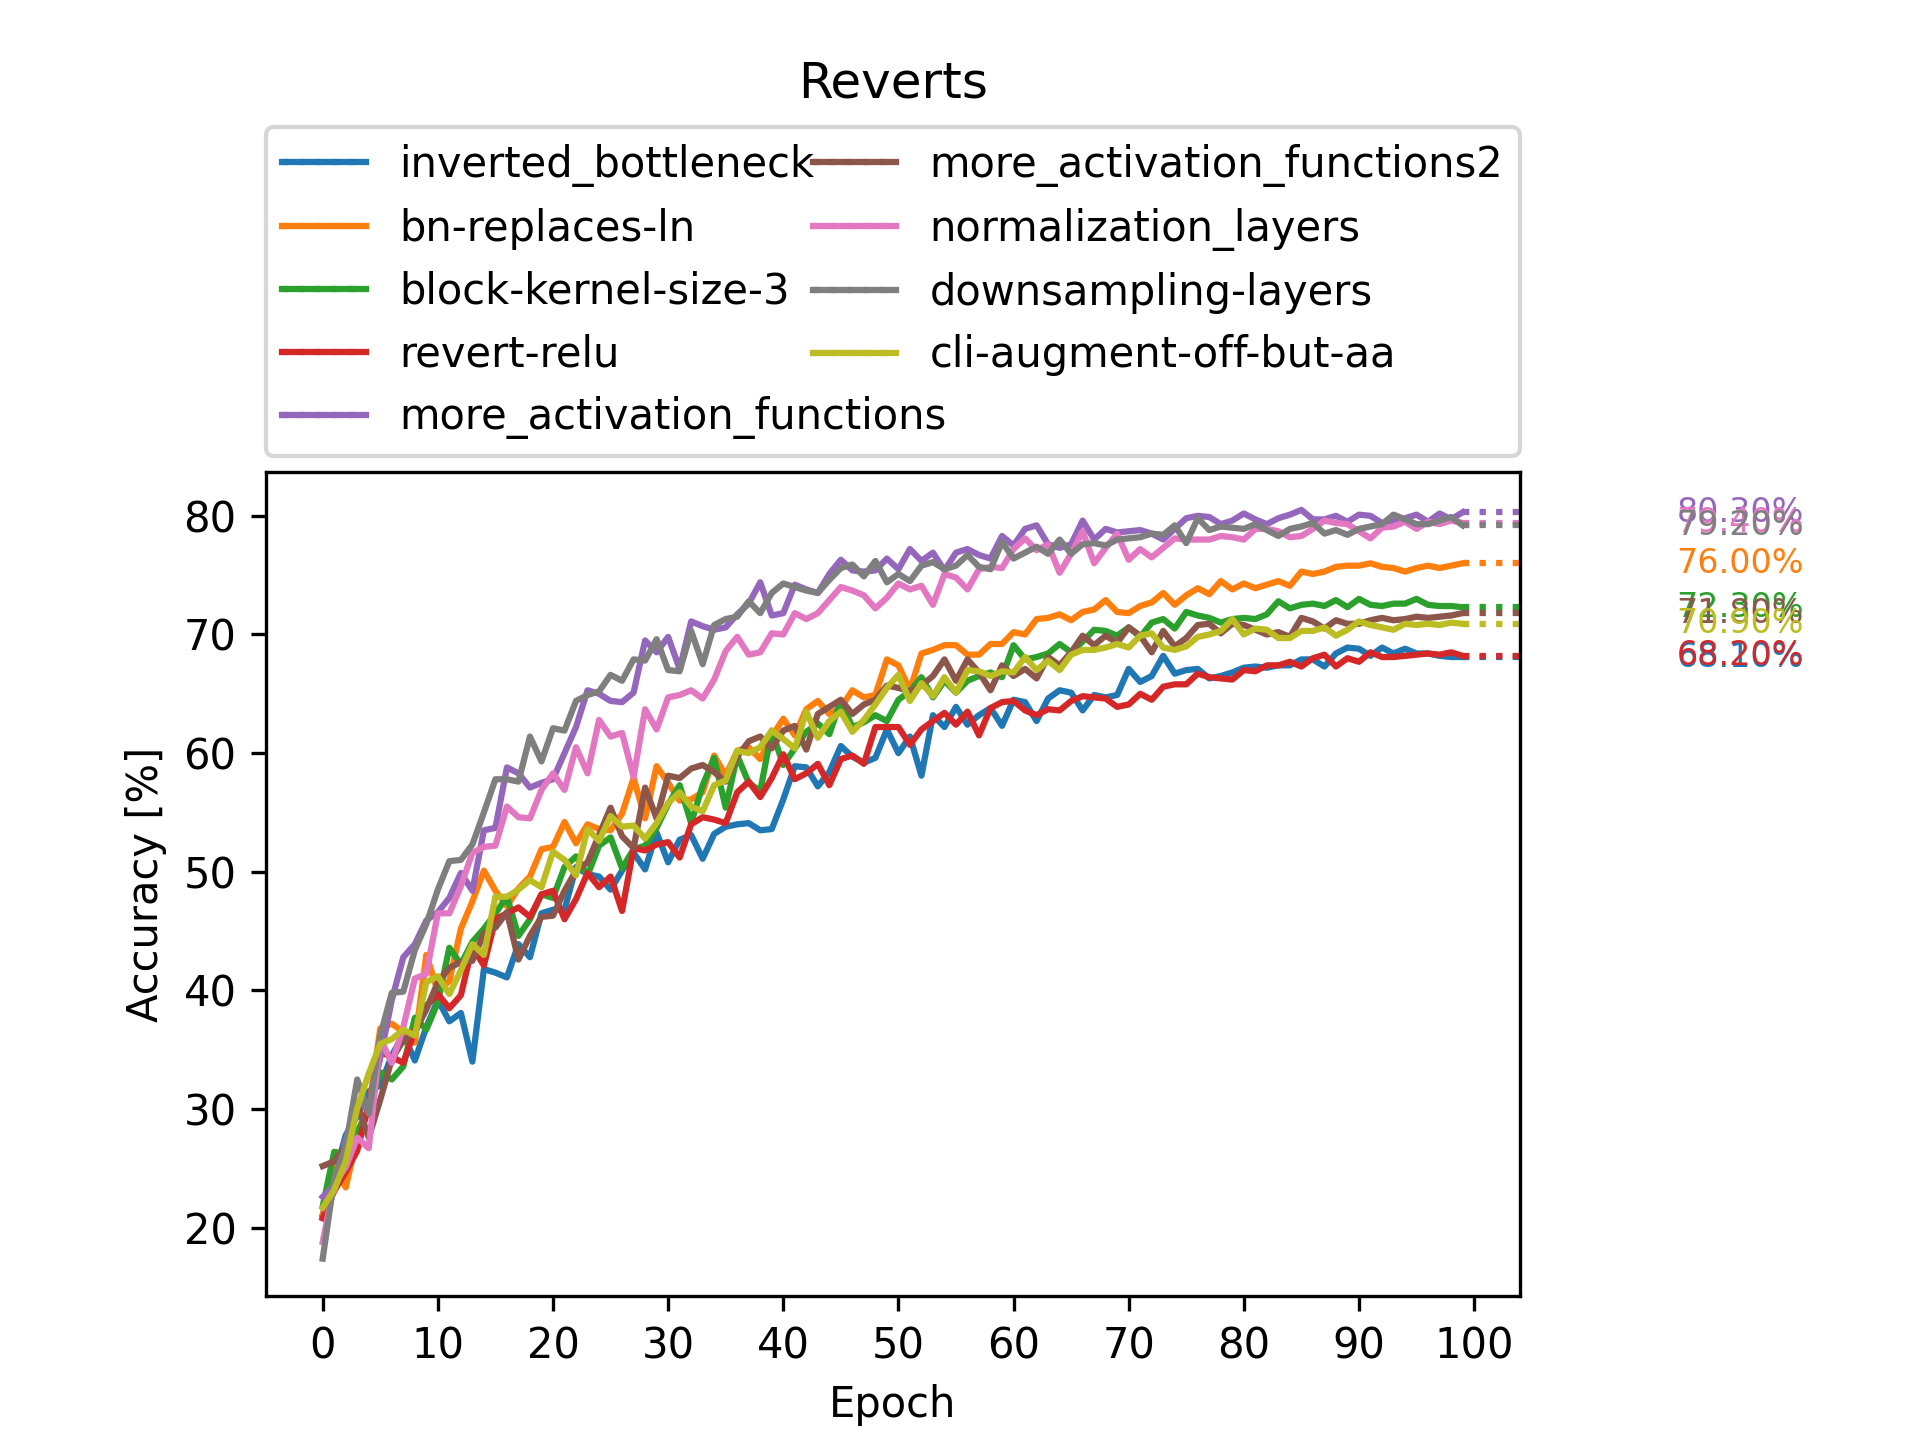
\includegraphics[width=0.8\textwidth]{images/reverts}
    \caption{Comparison of different reversions.}
    \label{fig:reverts}
\end{figure}

\textbf{GELU.} %
First up was reverting from the GELU activation function to ReLU\@.
This was a very quick and easy change, as there is only one line of code to change.
It is located in the class definition of \texttt{Block} in the \texttt{convnext.py} file.
All other changes are also done in the same file, so for brevity it will be omitted.
The resulting network performance is slightly lower than the baseline (\texttt{revert-relu}).

\textbf{From LN to BN.} %
The next change was reverting from their custom implementation of layer normalization to batch normalization.
This was also not too difficult, and we just exchanged the definition of the norm in the Block class with the PyTorch inbuilt BatchNorm.
Additionally, in the forward method the normalization and the first permutation swapped places.
The performance of the network significantly shot up to an impressive 76\% (\texttt{bn-replaces-ln}).

\textbf{Kernel Size.} %
The kernel size of the ConvNeXt network is per standard larger than in most other ConvNets.
We decreased the number from 7x7 back to the gold standard of 3x3, by adjusting the responsive parameter in the depthwise conv layer in the ConvNeXt blocks.
\begin{python}
self.dwconv = nn.Conv2d(dim, dim,kernel_size=3, padding=3, groups=dim)
\end{python}
With this change we achieved a maximum accuracy of 72.3\% so just a bit below the accuracy than that with larger kernels, which matches the Observations of the paper (\texttt{kernel\_size}).

\textbf{More Activation Functions.} %
In ConvNeXt, the ReLU activation functions of e.g.\ ResNeXt are replaced with GELU functions.
Furthermore, the authors reduced the number of activation functions to one per block.
To revert this change, we added two GELU function in each block such that there are three activation functions at all, one after the first two Conv Layers respectively and one at the end of each block (same as in the ResNet Block in figure 4 in the paper, just with GELU functions).
As a result we got a much higher accuracy of 80.3\% (\texttt{more\_activation\_functions}).
The training time per epoch stayed the same.
In an earlier tests without the normalization layer at the end of the block, the resulted accuracy was still increasing, but not that much (71.8\%) (\texttt{more\_activation\_functions2}).

\textbf{Inverted Bottleneck.} %
The principle of the inverted bottleneck is improving the result in the ConvNeXt paper by 0.7\%.
Instead of reducing the dimensions within a block, the dimensions are increased by a factor of four between the second and third Convolution Layer.
To revert this, we added a parameter \texttt{inverted\_bottleneck}
to be able to manipulate the factor and set it to one.
\begin{python}
# pointwise convolutions in the constructor of the block class
self.pwconv1 = nn.Linear(dim, inverted_bottleneck * dim)
self.pwconv2 = nn.Linear(inverted_bottleneck * dim, dim)
\end{python}
The result was in fact a significant lower accuracy of 68.1\% (\texttt{inverted-bottleneck}).

\textbf{Normalization Layers.}
In order to improve the performance, the number of normalization layers in ConvNeXt is minimized to one at each block.
We tested a model with three BatchNorm layers, as it is used in ResNet.
The only challenging part there is the calculation of the correct number of dimensions at each position in the model respectively.
To use the BatchNorm layers we surrounded them by permutation functions to have the dataflow in the correct shape.
The result looks like this for each added normalization layer (just with different factors for the dimensions in the initialization, as the dimensions are dependent of the position in the model):
\begin{python}
# in the constructor
# initialize BatchNorm Layer
self.std_norm1 = nn.BatchNorm2(inverted_bottleneck * dim)

# in the forward method
x = x.permute(0, 3, 1, 2)
x = self.std_norm1(x)
x = x.permute(0, 2, 3, 1)
\end{python}
Perhaps because of these measures, the training time increased greatly, by about an hour.
However, the performance drastically improved to 79.4\% (\texttt{normalization\_layers}).

\textbf{Larger Downsampling Kernels.}
Downsampling is done by convolution layers of kernel size 3x3 in ResNet, and 2x2 in Swin Transformers.
ConvNeXt got an improved accuracy with a kernel Size of 2x2 as a consequence, we tested a larger kernel size on our dataset.
As done in reverts before, we added a parameter (\texttt{downsample\_kernel\_size}) to the \texttt{create\_model} function and changed the line for the downsampling conv layers.
\begin{python}
nn.Conv2d(dims[i], dims[i + 1],
        kernel_size=downsample_kernel_size, stride=2)
\end{python}
After the training with extended kernel sizes in the downsampling layer, our accuracy went up to 79.2\% (\texttt{downsampling-layers}).

\textbf{ResNeXtify.}
The process of resnextifying includes transforming key features of the network, which make ConvNeXt to what it is.
Furthermore, many steps are related and dependent on these changes.
As reverting these would rather be part of investigating ResNeXt and too involved, we kept those reverts untouched.

Many reversions of the changes made in ConvNeXt lead to an increased accuracy.
Especially increased kernel size of the downsampling layers, multiple activation functions and BatchNorm layers increased the performance by almost incredible 10\%.
This leads to the question of generalizability of the results in ConvNeXt to other training data.

\section{Conclusion}\label{sec:conclusion}
The most surprising result from our experiments is the very high performance of finetuning.
Even if we just used the smallest network size with arbitrary hyperparameter choices and the smallest pretrained network, our performance was in the mid-nineties.
With the optimal choices we found it was close to 99\%.

Unfortunately, just using the network to train from scratch gives only acceptable performance even when using the insights we gained from experimenting with data augmentation.
Additionally, some reverts to the network architecture significantly improve the performance of the network.
Therefore, our findings in the network reversion chapters lead us to conclude that the choices made by the authors of the architecture only benefit the performance when using ImageNet1k.

However, one thing we did not experiment much on was the choice of hyperparameters.
Seeing the impact just the one configuration had, we conjecture that there could have been an even better configuration with much better results.
Unfortunately, we did not have the time to investigate this hunch further as our goal to reduce training time in the data augmentation chapter did not come to fruition.
Nonetheless, fidgeting with the way the images are transformed still proved valuable as we could significantly improve the network performance when using particular settings.
% could have played around more with hyperparameters
% Marcel: higher acc if changing back some parameters -> paper just optimized on specific dataset?
% Marcel: some optimizations could be reproduced, maybe more tests on different datasets necessary to improve acc in general?
\printbibliography
%%%%%%%%%%%%%%%%%%%%%%%%%%%%%%%%%%%%%%%%%%%%%%%%%%%%%%%%%%%%
\section*{Checklist}
 \begin{enumerate}


        \item For all authors\ldots
        \begin{enumerate}
            \item Do the main claims made in the abstract and introduction accurately reflect the paper's contributions and scope?
            \answerYes{}
            \item Did you describe the limitations of your work?
            \answerYes{}
            \item Did you discuss any potential negative societal impacts of your work?
            \answerNo{}
            \item Have you read the ethics review guidelines and ensured that your paper conforms to them?
            \answerNo{}
        \end{enumerate}


        \item If you are including theoretical results\ldots
        \begin{enumerate}
            \item Did you state the full set of assumptions of all theoretical results?
            \answerNA{}
            \item Did you include complete proofs of all theoretical results?
            \answerNA{}
        \end{enumerate}


        \item If you ran experiments\ldots
        \begin{enumerate}
            \item Did you include the code, data, and instructions needed to reproduce the main experimental results (either in the supplemental material or as a URL)?
            \answerYes{}
            \item Did you specify all the training details (e.g., data splits, hyperparameters, how they were chosen)?
            \answerYes{}
            \item Did you report error bars (e.g., with respect to the random seed after running experiments multiple times)?
            \answerNA{}
            \item Did you include the total amount of compute and the type of resources used (e.g., type of GPUs, internal cluster, or cloud provider)?
            \answerYes{}
        \end{enumerate}


        \item If you are using existing assets (e.g., code, data, models) or curating/releasing new assets\ldots
        \begin{enumerate}
            \item If your work uses existing assets, did you cite the creators?
            \answerYes{}
            \item Did you mention the license of the assets?
            \answerYes{}
            \item Did you include any new assets either in the supplemental material or as a URL?
            \answerNo{}
            \item Did you discuss whether and how consent was obtained from people whose data you're using/curating?
            \answerNo{}
            \item Did you discuss whether the data you are using/curating contains personally identifiable information or offensive content?
            \answerNo{}
        \end{enumerate}


        \item If you used crowdsourcing or conducted research with human subjects\ldots
        \begin{enumerate}
            \item Did you include the full text of instructions given to participants and screenshots, if applicable?
            \answerNA{}
            \item Did you describe any potential participant risks, with links to Institutional Review Board (IRB) approvals, if applicable?
            \answerNA{}
            \item Did you include the estimated hourly wage paid to participants and the total amount spent on participant compensation?
            \answerNA{}
        \end{enumerate}


    \end{enumerate}
\appendix
\section{Appendix}\label{sec:appendix}
\subsection{Visualization and comparison of filters}\label{subsec:filter-images}
Images of filters in the convolution layers are sometimes difficult to interpret, but still worth a glance.
In our case we focussed on differences between a pretrained ConvNeXt tiny model and our trained-from-scratch standard model with the settings we found out to be best in our scenario.
We also looked at differences between the models trained with our data only but with different parameters but could not find relevant differences there, which is why we will not present it here.
\begin{figure}[h]
    \centering
    \begin{minipage}[b]{0.49\textwidth}
        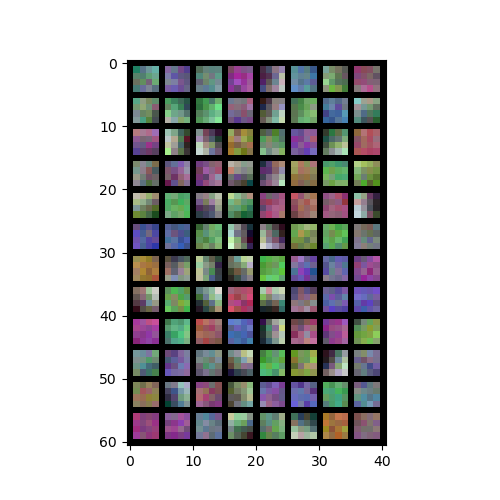
\includegraphics[width=\textwidth]{images/filters_layer0_from_scratch}
        \caption{Filters of self-trained network}
    \end{minipage}
    \hfill
    \begin{minipage}[b]{0.49\textwidth}
        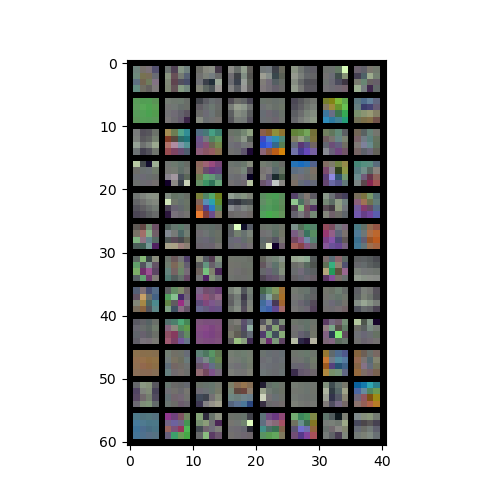
\includegraphics[width=\textwidth]{images/filters_layer0_pretrained}
        \caption{Filters of ConvNeXt tiny}
    \end{minipage}\label{fig:filters}
\end{figure}

The images show the filters with which every image is convolved with in the first layer of the network.
One point, that immediately stands out is the amount of colorful filters on the left, self-trained side and the many gray fields on the right, pretrained side.
Many filters seem to be dead, unused.

Besides that, filters on the left have rather flat and simple features, filters on the right are, if not completely gray, much more complex and show more fine-grained structures.
One possible reason for the grey fields is that filters were redundant, the network did more and more specialize on certain other filters and differentiated those.
The self trained model though had a much smaller pool of training data, and we also trained for a third amount of epochs in comparison.

\end{document}